\section{Teori \& bakgrund}
\subsection{Inledning}
% Bakgrund
Automatiska växellådor sitter idag i en mängd av olika fordon,
däribland en helt elektrisk buss under utveckling av Volvo.
För att bland annat köra på rätt växel, optimera motorns styrprogram
och operera olika bromsfunktioner % och vad mer/något mer?
mätes fordonets lutning.
För det ändamålet ska lutningsgivare användas.
Lutningsgivaren är en fristående modul som kommunicerar med styrdatorn via
Controller Area Network (CAN)-kommunikation.
Detta fungerar bra vid rörelse i konstant hastighet
men vid accelereration uppstår mätbrus och andra störningar.
Därför behövs en algoritm för att felkompensera dessa störningar.

% Räkna ut lutning med hjälp av moment
Ifall man inte har en lutningsgivare installerad i sitt fordon krävs ändå ett
sätt att räkna ut fordonets lutning.
Detta räknas ut med hjälp av vridmomentet i motorn.
Lutning kan approximeras med god säkerhet vid konstant hastighet men inbromsningar
skapar problem.
Vid inbromsning skapas en friktionskraft som måste tas till hänsyn.
Friktionskraftens moment beräknas med:
\begin{equation}
	M = r \cdot \mu \cdot \lVert F \rVert
\end{equation}
där $F$ är kraften, $r$ är radien, och $\mu$ är friktionskoefficienten
mellan bromsskivan och bromsbeläggen vilken kan variera mellan 0,2 och 0,4.
Därför uppstår en osäkerhet med att räkna ut lutningen utan lutningsgivare.
\autocite{lauri17}

%vad neuronnät är och vad de används till
Ett artificiellt neuronnät är en självlärande algoritm som inspirerats av
hur djurs hjärnor fungerar och kommunicerar.
Neuronnät kan användas för att klara av vissa problem som annars är svårlösta
med konventionella datalogiska metoder.
Ett neuronnät ``lär sig'', precis som vi gör, genom att observera.
Men för att ha avsedd funktion måste de tränas, alltså är arbete med neuronnät
uppdelat i två faser: en inlärningsfas och en tillämpningsfas där nätverket sedan
utför den ämnade uppgiften.
\autocite{copeland16}
Det är möjligt att sedan fortsätta träna nätverket
under användning, men oftast slutar man träna det när resultet är önskvärt.
\autocite{wiki-neuronnat}

\subsection{Piezoelektriska kristaller}
Piezoelektriska material ger upphov till
elektriska laddningar på deras yta under yttre mekaniskt tryck,
vilket kallas den direkta piezoelektriska effekten.
Det mekaniska arbete som utförs omvandlas till elektricitet, det omvända gäller
också, elektricitet omvandlas till mekansikt arbete i den omvända
piezoelektriska effekten i vilken kristallen deformeras.
\autocite{electronicdesign2016}
Piezoelektriska lutningsgivare använder elektriska signaler som är
inducerade via den piezoelektriska effekten från en piezoelektrisk kropp
under gravitationskraften från en tyngd.
Vinkeln mellan gravitationskraften och
riktningen på den piezoelektriska kroppens vibration
fås av att man mäter magnituden av kraftkomponenten i vibrationens riktning
och använder geometriska samband mellan dem.
\autocite{chiang00}

% Fel i piezokristaller
Felen i piezokristallerna härstammar från att signalen som orsakas av fordonets
lutning är väldigt svag.
När fordonet vibrerar orsakas störningar i signalen och eftersom den är så svag
påverkas den avsevärt.
Sedan finns det ett fel i uppskattningen av accelerationen.
Sensorn som mäter accelerationen använder tidsderivatan av hastigheten för
att räkna ut accelerationen.
Hastigheten mäts via ett kugghjul.
När sensorn i kugghjulet utsätts för viberationer kommer mätningen av
hastigheten att påverkas vilket ger opålitliga resultat.
Detta fel uppstår både vid lutningsapproximation med lutningsgivare likväl som utan.
Dock är felet lättare att lösa när lutningsgivare används.
Dessa anledningar gör att lutningsgivare är fördelaktiga att använda.

\subsection{Artificiella neuroner}
% Figur för neuron
\begin{figure}
	\centering
	\begin{tikzpicture}[
			init/.style={draw,circle,inner sep=2pt,font=\Huge,join = by -latex},
		squa/.style={draw,inner sep=2pt,font=\Large,join = by -latex},
		start chain=2,node distance=13mm]
	\node[on chain=2] (x2) {$x_2$};
		\node[on chain=2,join=by o-latex] {$w_2$};
		\node[on chain=2,init] (sigma) {$\displaystyle\Sigma$};
		\node[on chain=2,squa,label=above:{\parbox{2cm}{\centering Aktiverings-\\ funktion}}] {$\phi$};
		\node[on chain=2,label=above:Output,join=by -latex] {$y$};
		\begin{scope}[start chain=1]
			\node[on chain=1] at (0,1.0cm) (x1) {$x_1$};
			\node[on chain=1,label=above:Vikter,join=by o-latex] (w1) {$w_1$};
		\end{scope}
		\begin{scope}[start chain=3]
			\node[on chain=3] at (0,-1.0cm) (x3) {$x_3$};
			\node[on chain=3,join=by o-latex] (w3) {$w_3$};
		\end{scope}
		\node[label=above:\parbox{2cm}{\centering Bias, $b$}] at (sigma|-w1) (b) {};
		\draw[-latex] (w1) -- (sigma);
		\draw[-latex] (w3) -- (sigma);
		\draw[-latex] (b) -- (sigma);
		\draw[decorate,decoration={brace,mirror}] (x1.north west) -- node[left=10pt] {Inputs} (x3.south west);
	\end{tikzpicture}
	\caption{Schematisk skiss över en neuron.}
	\label{fig:neuron}
\end{figure}

% Figur för sigmoidfunktionens graf
\begin{figure}
	\centering
	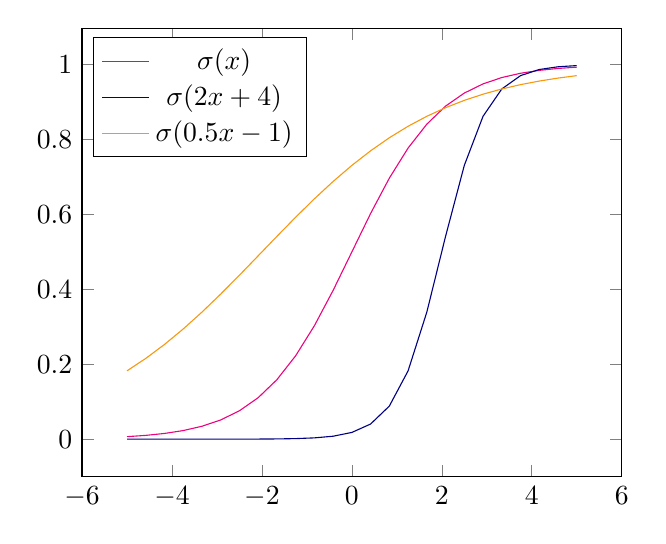
\begin{tikzpicture}
		\begin{axis}[legend style={at={(0.02,0.98)},anchor=north west},
			legend entries={$\sigma(x)$, $\sigma(2x + 4)$, $\sigma(0.5x - 1)$}]
			\addplot[RubineRed] {(1)/(1+e^-x)};
			\addplot[NavyBlue] {(1)/(1+e^(-2*x+4))};
			\addplot[YellowOrange] {(1)/(1+e^(-0.5*x-1))};
		\end{axis}
	\end{tikzpicture}
	\caption{Aktiveringsfunktionen sigmoid. \label{fig:sigmoid}}
\end{figure}

% Neuronen
En artificiell neuron tar in en eller flera inputs och producerar en output $y$,
se figur~\ref{fig:neuron}.
Varje input, $x_n$, är tilldelad en \emph{vikt}, $w_n$.
Utöver det har varje neuron en \emph{bias}, $b$.
Neuronens inputs, $x_1,x_2, \dotsc, x_n$, vikterna, $w_1, w_2, \dotsc, w_n$,
och biasen, $b$, ger en s.k. \emph{weighted input}, $z$:
\begin{equation}
	z \equiv \sum_n w_n x_n + b
\end{equation}
Neuronens output är resultatet av en aktiveringsfunktion för $z$, $\phi(z)$.
Aktiveringsfunktionen kan vara vad som helst så länge den är deriverbar,
men olika funktioner ger olika bra resultat.
Sigmoidfunktionen, $\sigma(z)$, är ett exempel på en sådan aktiveringsfunktion
och ser ut som:
\begin{equation}
	\sigma(z) \equiv \frac{1}{1 + e^{-z}}
\end{equation}
Dess värdemängd är normaliserad från 0\,till\,1, se figur~\ref{fig:sigmoid}.
Om $z$ är ett stort positivt tal kommer $ \sigma(z) \approx 1 $,
medan om $z$ är ett stort negativt tal så kommer $ \sigma(z) \approx 0 $.
Grafens lutning påverkas av vikterna medan biasen förskjuter hela kurvan i x-led.
Med sigmoidfunktionen blir neuronens output alltså $ \sigma(\sum_n w_n x_n + b) $.
\autocite{nielsen15}

\subsection{Neuronnätsarkitektur}
\begin{figure}
	\centering
	\def\layersep{2.5cm}
	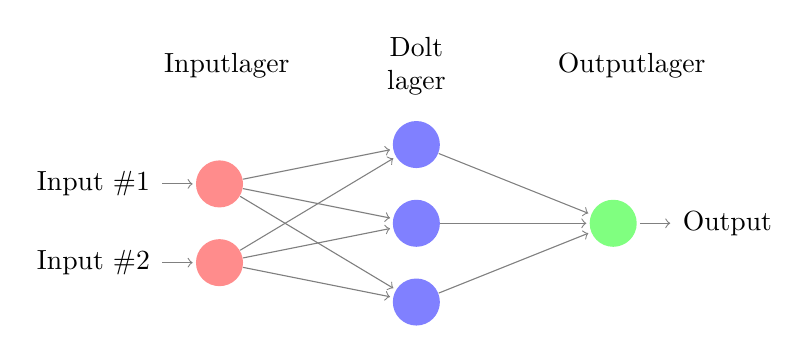
\begin{tikzpicture}[shorten >=1pt,->,draw=black!50, node distance=\layersep]
		\tikzstyle{every pin edge}=[<-,shorten <=1pt]
		\tikzstyle{neuron}=[circle,fill=black!25,minimum size=17pt,inner sep=0pt]
		\tikzstyle{input}=[neuron, fill=red!45];
		\tikzstyle{output}=[neuron, fill=green!50];
		\tikzstyle{hidden neuron}=[neuron, fill=blue!50];
		\tikzstyle{annot} = [text width=4em, text centered]

		\foreach \name / \y in {1,...,2}
			\node[input, pin=left:Input \#\y] (I-\name) at (0,-\y) {};
		\foreach \name / \y in {1,...,3}
			\path[yshift=0.5cm]
				node[hidden neuron] (H-\name) at (\layersep,-\y cm) {};
		\node[output,pin={[pin edge={->}]right:Output}, right of=H-2] (O) {};
		\foreach \source in {1,...,2}
			\foreach \dest in {1,...,3}
				\path (I-\source) edge (H-\dest);
		\foreach \source in {1,...,3}
			\path (H-\source) edge (O);

		\node[annot,above of=H-1, node distance=1cm] (hl) {Dolt lager};
		\node[annot,left of=hl] {Inputlager};
		\node[annot,right of=hl] {Outputlager};
	\end{tikzpicture}
	\caption{Exempel på feed-forward neuronnät. \label{fig:network}}
\end{figure}

Neuronnät består av flera neuroner som alla är sammankopplade, se figur~\ref{fig:network}.
I ett s.k. \textit{feed-forward} neuronnät får varje neuron inputs från
varenda neuron i det tidigare lagret.
Inputlagret får sina inputs direkt.
Det dolda lagret kallas så eftersom det inte är uppenbart hur det fungerar;
så vitt vi vet skulle det kunna använda sitt brutna ben
för att skyffla informationen framåt.
Outputlagrets aktiveringar blir resultatet av neuronnätet.
Medan antalet input- och outputneuroner otvetydligt kan bestämmas
från formen av ens träningsdata,
så finns bara empiriskt deriverad heuristik för strukturen på ens dolda lager.
Exempel på nackdelar med fler neuroner är längre träningstider
och behovet av mer träningsdata.
Neuronnät är specifika för en uppgift och en arkitektur som
fungerar bra i ett fall behöver inte nödvändigtvis göra det i ett annat.
\autocite{nielsen15}

\subsection{Stochastic gradient descent}
% Förlustfunktionen
Med hjälp av en slät funktion för hur väl nätet approximerar träningsdatan
kan man korrelera små ändringar i vikter och biases
till små förbättringar i prestandan.
Den \emph{kvadratiska förlustfunktionen} är en sådan funktion:
\begin{equation} \label{eq:cost}
	C(w, b) \equiv \frac{1}{2n} \displaystyle\sum_x \lVert y(x) - a \rVert^2
\end{equation}
där $ w $ är alla vikter i nätet, $ b $ är alla biases,
$ n $ är antalet träningsindata, $ a $ är en vektor med utdata när $ x $ är indata
och summan är över all träningsindata $ x $.
Man ser att $ C(w, b) $ är icke-negativ då varje term i summan är positiv.
Dessutom är förlusten $ C(w, b) $ liten, det vill säga $ C(w, b) \approx 0 $,
när $ y(x) $ är ungefär lika med utdatan, $ a $, för alla träningsindata, $ x $.
Målet med träningsalgoritmen blir då att minimera $ C(w, b) $.

% Figur för gradient descent
\begin{figure}
	\centering
	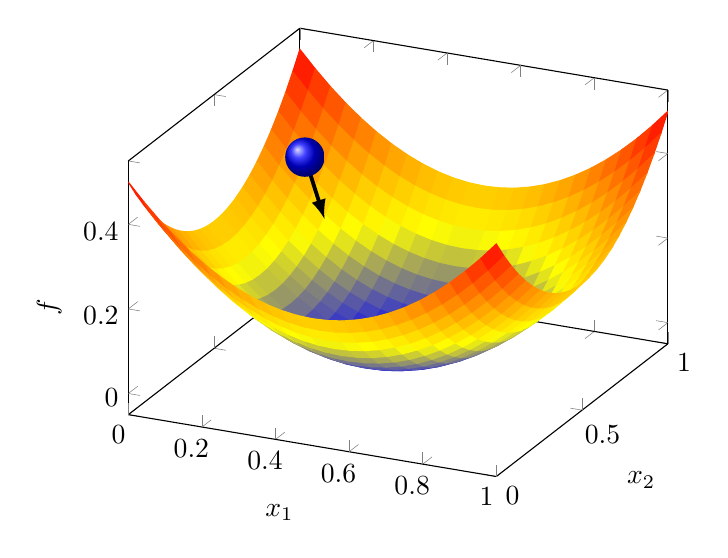
\begin{tikzpicture}
		\begin{axis}[domain=0:1,xlabel={$x_1$},ylabel={$x_2$},zlabel={$f$}]
			\addplot3[surf,shader=flat] {(x-0.5)^2 + (y-0.5)^2};
			\draw[->,line width=0.004\linewidth,>=latex] (axis cs:0.2,0.6,0.4) -- (axis cs:0.3,0.5,0.3);
			\node[circle,shading=ball,minimum width=0.5cm] (ball) at (axis cs:0.2,0.6,0.4) {};
		\end{axis}
	\end{tikzpicture}
	\caption{Gradient descent kan efterliknas vid en boll som rullar nerför en dal.}
	\label{fig:descent}
\end{figure}

En algoritm för det är \emph{gradient descent}.
Om man föreställer sig en funktion $ f(x_1, x_2) $ som en dal,
se figur~\ref{fig:descent},
säger intuition att en boll skulle rulla nerför sluttningen till botten.
Vi kan simulera detta genom att räkna ut gradienten av $ f $.
Gradienten av $ f $, $ \nabla f $, vid en punkt är en vektor
som pekar i riktningen av den brantaste lutningen vid den punkten:
\begin{equation}
	\nabla f = \begin{bmatrix} \frac{\partial f}{\partial x_1} & \frac{\partial f}{\partial x_2} \end{bmatrix}^{T}
\end{equation}
där $ \partial f / \partial x_i $ är den partiella derivatan
som beskriver hur snabbt $ f $ växer med avseende på variablen $ x_i $.
Vi kan minska $ f $ genom att gå i riktningen av den negativa gradienten:
\begin{equation}
	x \leftarrow x - \eta \nabla f(x)
\end{equation}
där $ \eta $ är inlärningshastigheten,
en positiv skalär som bestämmer längden av steget.
Genom att generalisera det till flera dimensioner kan vi
applicera det på neuronnät:
\begin{align}
	w_k &\leftarrow w_k - \eta \frac{\partial C}{\partial w_k} \\
	b_l &\leftarrow b_l - \eta \frac{\partial C}{\partial b_l}
\end{align}

Då förlustfunktionen i ekvation~\eqref{eq:cost} är ett genomsnitt av
förlusterna $ C_x = \frac{\lVert y(x) - a \rVert^2}{2} $ för individuella träningsexempel
kan det ta lång tid att beräkna gradienten med ett stort antal träningsindata.
\emph{Stochastic gradient descent} uppskattar $ \nabla C $ genom att
sampla en \emph{minibatch} av likformigt slumpade exempel
$ \mathbb{B} = \left\{ x_1, \dotsc, x_{m'} \right\} $ från träningsindatan
och räkna ut gradienten från dem:
\begin{equation}
	\nabla C \approx \frac{1}{m'} \sum^{m'}_{i=1} \nabla C_{x_i}
\end{equation}
med exempel från minibatchen $ \mathbb{B} $.

\section{Syfte}
Syftet med undersökningen är att ta fram och utvärdera en algoritm med
artificiella neuronnät som felkompenserar lutningsgivare i elbussväxellådor.

\section{Frågeställningar}
Vi vill undersöka\ldots
\begin{itemize}
	\item Varför råsignalen från lutningsgivaren blir opålitlig.
	\item Hur nätverket ska vara konfigurerat för att felkompensera; vilka inputs,
		outputs, antal neuroner, hidden layers och feed-/cascade-forward?
	\item Hur väl det fungerar att felkompensera med neuronnät.
\end{itemize}
